\documentclass[12pt,a4paper]{article}
\usepackage{appendix}
\usepackage[utf8]{inputenc}
\usepackage[french]{babel}
\usepackage[T1]{fontenc}
\usepackage{amsmath}
\usepackage{amsfonts}
\usepackage{amssymb}
\usepackage{graphicx}
\usepackage[left=2cm,right=2cm,top=2cm,bottom=2cm]{geometry}
\usepackage{ccaption}
\author{Malenfer François, Carbonneau Danaël}

\usepackage[Glenn]{fncychap}

\usepackage{fancybox}

\usepackage{multicol}
\usepackage[hidelinks]{hyperref}

\usepackage[dvipsnames]{xcolor}
\usepackage{tcolorbox}
\usepackage{listings}
\usepackage{algorithm,algorithmic}



	
	
\definecolor{darkWhite}{rgb}{0.94,0.94,0.94}
 
\lstset{
  aboveskip=3mm,
  belowskip=-2mm,
  backgroundcolor=\color{darkWhite},
  basicstyle=\footnotesize,
  breakatwhitespace=false,
  breaklines=true,
  captionpos=b,
  commentstyle=\itshape \color{teal},
  extendedchars=true,
  framexleftmargin=16pt,
  framextopmargin=3pt,
  framexbottommargin=6pt,
  frame=tb,
  keepspaces=true,
  keywordstyle=\bfseries \color{orange},
  otherkeywords={module,open,Int32,val},
  language=caml,
  morekeywords={*,...},
  numbers=left,
  numbersep=10pt,
  numberstyle=\tiny\color{teal},
  rulecolor=\color{black},
  showspaces=false,
  showstringspaces=false,
  showtabs=false,
  stepnumber=1,
  stringstyle=\color{gray},
  tabsize=4,
  title=\lstname,
}	
	
	
	
	
\usepackage{enumitem}
\usepackage{pifont}
\setitemize[1]{font=\bfseries, label= \color{teal} \ding{227}  }
\setitemize[0]{font=\bfseries, label= \color{olive} \ding{216}  }


\begin{document}


\begin{titlepage}
\newcommand{\HRule}{\rule{\linewidth}{0.5mm}}



\center 
\bigskip
\textsc{\LARGE\textbf{
\color{teal}Sorbonne Université}
}
 \\[4cm]
 {\color{Bittersweet}\HRule} \\[0.4cm]
{ \huge \bfseries \color{darkgray} Devoir de Programmation \\[0.15cm] }
\textbf{Algorithmique Avancée}
{\color{Bittersweet}\HRule} \\[0.5cm]

{\color{darkgray} François Malenfer (28706664), Danaël Carbonneau (28709878)} \\[3cm]

\begin{huge}
{\fontfamily{lmtt}\selectfont
Implémentation de structures de données de recherche (en OCaml)\cite{leroy3ocaml}
}
\end{huge}


\vfill

\textit{Enseignant : Antoine Genitrini}

Master Informatique, Semestre 1, septembre - janvier 2023 - 2024 \\ [1cm]

\end{titlepage}


\setcounter{tocdepth}{2}
\tableofcontents


\newpage
 \section{Échauffement}
Le code correspondant à cette section se trouve dans le fichier \textit{int128.ml}. En plus des fonctions demandées par le sujet, nous y avons ajouté d'autres fonctions utilitaires pour manipuler les entiers 128 dans la suite du projet : 

\begin{description}

\item[\textit{of\_str}] convertit une chaîne de caractère en entier 128.
\item[\textit{to\_str}] convertit un entier 128 bits en une chaîne de caractères.
\item[\textit{list\_of\_file}] permet de récupérer une liste d'entiers 128 bits depuis un fichier présentant des clés au bon format.
\end{description}

\subsection{Représentation d'une clé 128 bits}

OCaml nous donne accès au module Int32, qui permet d'avoir des entiers codés sur exactement 32 bits. Nous allons les utiliser dans un tuple de 4 entiers de taille 32 bits qui font la décomposition de notre entier 128 bits.

\medskip

\begin{lstlisting}
open Int32;;
type entier128 = (Int32.t * Int32.t * Int32.t * Int32.t);;

\end{lstlisting} \medskip


Pour implémenter nos prédicats, nous avons choisi d'écrire une fonction \textit{compare}, qui compare des bits de poids forts vers ceux de poids faible les entiers 32 bits qui composent nos entier 128 bits. Ce choix nous permet de factoriser le code pour nos deux prédicats de comparaison.

\medskip \begin{lstlisting}
let cmp (cle1 : t) (cle2 : t) : int = 
  let (a1, b1, c1, d1) = cle1 and (a2, b2, c2, d2) = cle2 in 
  if a1=a2 then 
    if b1=b2 then 
      if c1 = c2 then
        (Int32.unsigned_compare d1 d2)
      else
        (Int32.unsigned_compare c1 c2)
    else
      (Int32.unsigned_compare b1 b2) 
  else 
    (Int32.unsigned_compare a1 a2)
\end{lstlisting} 

\subsection{Le prédicat inf}

Ce prédicat peut être implémenté en vérifiant si le résultat de compare est négatif. Nous avons également implémenté une fonction \textit{inf2}, qui permet de manipuler des clés sous forme de type option.

\medskip \begin{lstlisting}
let inf (cle1 : t) (cle2 : t) : bool = (cmp cle1 cle2) < 0
\end{lstlisting} 

\subsection{Le prédicat eg}
De manière analogue, le prédicat peut être implémenté en vérifiant si le résultat de compare est nul.

\medskip \begin{lstlisting}
let inf (cle1 : int128) (cle2 : int128) : bool = (cmp cle1 cle2) = 0
\end{lstlisting} \medskip



 \section{Structure 1 : Tas priorité min}

Dans cette section, nous allons étudier deux manières d'implémenter des tas minimum : une utilisant une structure de tableau, ce qui est la manière la plus usuelle de représenter les tas minimum, et une utilisant une structure arborescente, permettant d'implémenter nos algorithmes dans un style purement fonctionnel.
Le code se trouve dans les fichiers \textit{tas\_min\_tab.ml} et \textit{tas\_min\_arbre.ml}. 

Nos structure sont les suivantes : 

\bigskip \begin{lstlisting}
(*indice dernier element * taille du tableau * tableau*)
type heapArray = int ref * int ref * (Int128.t option) Array.t;;

(* Noeud of  rang * ndescendants * elt * fg * fd *)
type  heapTree = E | L of Int128.t | N of int * int *  Int128.t *  heapTree *  heapTree;;
\end{lstlisting} \bigskip

Le tas sous forme de tableau est représenté à l'aide de types option, ce qui permet de ne pas devoir le copier dans un tableau plus petit à chaque suppression, mais également de pouvoir l'agrandir d'un étage à chaque fois qu'on atteint la taille limite du tableau (ce qui permet d'éviter de trop faire cette couteuse opération de copie) : on rend possible le fait d'avoir des cases vides dans le tableau. Les deux entiers contenus dans la structure sont des références afin de rester cohérents avec la mutabilité du tableau (on veut pouvoir leur réaffecter de nouvelles valeurs). Dans le tableau, l'arbre est représenté en considérant le lien suivant entre les cases : L'indice d'un père, par rapport à son fils d'indice i est $(i-1)/2$, l'indice du fils droit d'un père i est $2*i +1$, celui de son fils gauche est $2*i+2$.


Pour le tas sous forme d'arbre, nous avons choisi de faire un constructeur feuille permettant de savoir facilement, dans nos match, lorsque nous arrivons au bout de l'arbre. Afin de pouvoir naviguer dans l'arbre, il nous est également nécessaire de retenir plusieurs informations sur chaque nœud afin de nous aiguiller lors des ajouts et des suppressions : le rang et le nombre de descendants. Cette manière d'implémenter la structure s'inspire de celle présentée dans \textit{Purely functionnal data structures}, de Chris Okasaki \cite{DataStructure} pour les \textit{Leftist Heaps}, notamment pour la notion de rang, qui est la distance la plus courte d'un nœud vers un nœud vide (en nombre de nœuds). 


Nos deux structures, en plus des fonctions de manipulations demandées par le sujet, sont munies d'une fonction \textit{to\_dot}, qui permet, grâce au langage dot, de visualiser sous forme d'arbre le résultat de nos opérations. Les différents arbres obtenus sont dans le dossier \textit{Images/graphes}

\subsection{Implémenter les 3 fonctions fondamentales d'un tas min}

\subsubsection{Tas min sous forme de tableau}

Pour notre fonction \textit{Ajout}, il suffit de faire une insertion à la fin du tableau grâce à l'indice maintenu (opération $O(1)$), puis de remonter dans l'arbre afin de faire des permutations tant que la clé du fils est plus petite que celle du père. 

Pour \textit{SupprMin}, on récupère le premier élément du tableau, qui est, par définition et construction du tas, le minimum dans la structure, puis on récupère l'élément se situant à la dernière case où un élément a été inséré, on le met dans la case d'indice 0, et on descend dans l'arbre en échangeant la clé courante avec celle de son fils ayant le plus petit élément (s'il est inférieur), puis en recommençant, si besoin, dans le fils où on a fait l'insertion.

Pour \textit{AjoutsIteratifs} nous pouvons créer un tas vide de la taille de notre liste, puis y faire tous nos ajouts avec la fonction définie précédemment


\subsubsection{Tas min sous forme d'arborescence}

Pour notre fonction \textit{Ajout}, on parcourt l'arbre à l'aide du rang pour trouver le prochain nœud vide en faisant le long du parcours les inversions de clés permettant de garder la propriété minimale du tas

Pour \textit{SupprMin}, on parcourt l'arbre à l'aide du rang et du nombre de descendants pour trouver le dernier nœud ajouté dans le tas, losqu'on la trouvé, on fait remonter l'élément et on fait appel aux fonctions \textit{reeq\_tas\_gauche} et \textit{reeq\_tas\_droite} pour replacer correctement l'élément remonté (toujours le minimum du tas récupéré avec l'appel récursif) dans le tas afin de garder sa propriété minimale

Pour \textit{AjoutsIteratifs}, il suffit de parcourir la liste et d'ajouter ses éléments uns par uns au tas (en commençant avec un tas vide).

\subsection{Construction}

Un algorithme permettant de construire un tas en temps constant a été présentée par l'informaticien Robert W. Floyd en 1964 dans une communication de l'Association for Computing Machinery\cite{ACM}, puis reprise, notamment, par Donald E. Knuth dans \textit{The Art of Computer Programming, Vol. III Sorting and Searching}\cite{KnuthHeap}.


\begin{algorithm}
\caption{Heapify}
\begin{algorithmic}
\REQUIRE{n un tas}
\IF{ n n'est pas une feuille et qu'un de ses fils est plus petit que la clé de n}
 	\STATE f est le fils de n avant la clé la plus petite
 	\STATE interchanger cle(f) et cle(n)
 	\STATE heapify (f)
\ENDIF
\end{algorithmic}
\end{algorithm}

\begin{algorithm}
\caption{Construction}
\begin{algorithmic}
\REQUIRE{l, une liste de clés}
\STATE t = transformation de l en une structure d'arbre parfait

\FOR{k un nœud dans t en partant du dernier dans l'arbre parfait jusqu'à la racine}

\STATE heapify (k)
	
\ENDFOR
\end{algorithmic}
\end{algorithm}

Le principe est donc de d'abord s'assurer de la structure de l'arbre globale (sous forme d'arbre parfait tassé à gauche), puis de partir des feuilles pour "heapify" (faire tas) les sous arbres qui composent le résultat final dans un parcours Bas Haut Droite Gauche.

La forme de cet algorithme s'adapte assez bien au style de programmation fonctionnel dans la mesure où les modifications sont locales à l'arbre étudié au moment où on le \textit{heapify}.


\subsubsection{Implémentation par tableau}

Pour l'implémentation par tableau, il nous suffit de convertir la liste en tableau (par une primitive fournie par le module \textit{Array}), puis de faire les remontées grâce aux indices depuis la fin de ce dernier.

\subsubsection{Implémentation par arborescence}

Pour l'arborescence, bien que les appels à \textit{heapify} soient assez simples à situer (dès qu'on créé un nouvel arbre tassé à gauche, on le heapify, ce qui forme alors bien un tas, qu'on peut retourner), la question de créer un arbre parfait tassé à gauche depuis une liste est moins évidente.

Pour résoudre ce problème, nous utilisons le fait qu'à un nombre d'éléments donné, il n'y a qu'une seule forme d'arbre parfait tassé à gauche possible : il nous est possible donc, de savoir, pour un nœud donné, en fonction de la taille qui a été passée en argument, de savoir la taille de sa descendance droite et de sa descendance gauche : on peut alors faire deux appels récursifs demandant cette taille de tas pour obtenir deux fils aux tailles souhaitées : de là, il nous suffit de les combiner avec un nouvel élément tiré de la liste passée en argument, puis de faire appel à \textit{heapify} sur notre nouveau nœud, pour obtenir un tas minimal de la taille souhaitée.

La fonction \textit{construction} consiste alors à récupérer la taille de la liste, puis faire un appel à \textit{make\_tas}.

\bigskip \begin{lstlisting}
let rec make_tas (li : Int128.t list) (taille : int) :  
	(heapTree * Int128.t list )= 
  if taille = 0 || taille < 0 then (E,li)
  else if taille = 1 then
    (*Cas d'arret : on veut faire un tas de taille 1, on renvoie une feuille du 1er element de la liste et le reste *)
  else
    let hauteur = log2 taille in
    let hauteur_prec = hauteur -1 in
    let reste = taille - ((two_pow hauteur)-1) in 
    if reste < ((two_pow hauteur)/2) then
      let nb_elem_gauche = reste+ (((two_pow (hauteur_prec+1)) -1)/2) in
      let nb_elem_droite = (((two_pow (hauteur_prec+1)) -1)/2) in
      let (fg,lr) = make_tas li nb_elem_gauche in
      let (fd,lr2) = make_tas lr nb_elem_droite in
      match lr2 with 
      | [] -> failwith "invalid argument"
      | h::tl -> let hp =  N( (min (rank fg) (rank fd)) +1, taille -1, h, fg, fd) 
      	in ( (heapify hp), tl)  
    else
      let nb_elem_gauche = ((two_pow hauteur)/2) + (((two_pow (hauteur_prec+1)) -1)/2) 
      in
      let nb_elem_droite = (((two_pow (hauteur_prec+1)) -1)/2) + (reste - ((two_pow hauteur)/2))
      in
      (*meme principe que dans l'autre cas, mais avec les nombres d'elements calcules ici *)

\end{lstlisting} \bigskip


\subsection{Union}

Pour réaliser l'union en temps linéaire de deux tas, il suffit de mettre tous leurs éléments dans une même liste (ou un même tableau), puis de faire appel à construction sur cette liste nouvellement créée.

\subsubsection{Implémentation par tableau}

On fait la concaténation des deux tableaux avec la primitive du module \textit{Array} \textit{Array.append}, sur laquelle on reprend le même fonctionnement que pour construction (on remonte depuis les feuilles pour \textit{heapify} les nœuds sur le chemin vers la racine).


\subsubsection{Implémentation par arbre}

Pour pouvoir utiliser notre fonction construction, il nous faut construire une liste en temps linéaire contenant tous les éléments des deux listes. Nous avons écrit, pour cela, une fonction \textit{heap\_to\_list} qui permet de transformer un tas en une liste de ses clés en temps linéaire. Ainsi, pour faire l'union, on relie nos deux tas par un nœud "fantôme" (\textit{N(0,0,(0l,0l,0l,0l))}) qui sera en tête de la liste obtenue par un appel à \textit{heap\_to\_list} . Il suffit alors d'appeler \textit{construction} sur la liste privée de cette tête.


\subsection{Preuves des différentes complexités}

\subsubsection{Ajout}

\subparagraph{Tas sous forme de tableau}

En maintenant un indice contenant la dernière case où il est possible d'ajouter, en supposant que le tableau a la bonne capacité, on parvient à faire l'ajout en $O(log (n) ) $ : insérer un élément se fait en $O(1)$, puis on remonte, au pire cas, la hauteur du tas, ce qui se fait en $O(log (n))$.

\subparagraph{Tas sous forme d'arborescence}

À l'aide du système d'aiguillage permis par le fait de retenir le rang (dont les opérations de vérification se font en temps constant), on parcourt notre tas de haut en bas avec à chaque fois un appel récursif vers le bon fils où se fera l'ajout. Après cet appel récursif, on reconstruit un nœud en faisant les rééquilibrages au fur et à mesure. Notre complexité en nombre de comparaisons se fait donc bien en temps $O(log (n))$. 


\subsubsection{SupprMin}

\subparagraph{Tas sous forme de tableau}

De même que pour l'ajout, on fait des opérations en O(1) sur le tableau pour le retrait, puis le rééquilibrage se fait en parcourant une branche du tas, donc en $O(log (n))$.
\subparagraph{Tas sous forme d'arborescence}


À l'aide de notre système d'aiguillage, cette fois-ci basé sur le rang et le nombre de descendants (dont les opérations de vérification se font en temps constant), on parcourt notre tas de haut en bas avec à chaque fois un appel récursif vers le bon fils où se fera la suppression. Après cet appel récursif, on reconstruit un nœud en faisant les rééquilibrages au fur et à mesure. Notre complexité en nombre de comparaisons se fait donc bien en temps $O(log (n))$. 



\subsubsection{Ajouts itératifs}

Dans nos deux implémentations, on itère sur une liste de taille n en faisant n ajouts chacun en $O( log (n))$, on a bien une complexité théorique majorée par $O(n log(n))$.
\subsubsection{Construction}

Dans l'article \textit{An Average Case Analysis of Floyd's Algorithm to Construct Heaps}\cite{Doberkat}, Ernst E. Doberkat nous présente une analyse de la complexité de l'algorithme de Floyd, sur laquelle nous allons nous baser.

Posons $h$ la hauteur du tas, c'est à dire qu'il contient des niveaux allant de $0$ à $h - 1$. Dans le pire des cas, chaque opération bubble down (effectuée une fois pour chaque nœud) va se faire sur la distance du nœud aux feuilles, c'est à dire $h - 1 - h(x)$, où $h(x)$ est la hauteur relative du nœud x par rapport à la racine.

\newpage
Le coût total pour tous les nœuds est donc majoré par 

\begin{align}
C &= \sum_{i = 0}^{h-1} 2^i (h - 1 - i)\\
&=  \sum_{j = 0}^{h-1} 2^{h-1-j} j\\
&= 2^{h-1} \sum_{j=0}^{h-1} 2^{-j} j\\
&= 2^{h-1} \sum_{j=0}^{h-1} j \frac{1}{2^j} \\
&= O(2^{h-1})\\
&= O(n)
\end{align}

\begin{enumerate}[label=(\arabic*)]
\item $2^i$ est le nombre de nœuds à l'étage i dans le tas, on le multiplie par le coût maximum pour un nœud de cet étage
\item On pose $j = h-1 -i \iff i = h-1 -j$
\item On sort $2^{h-1}$ de la somme
\item $2^{-j} = \frac{1}{2^j}$, propriété des puissances
\item la série $\sum_{i = 0}^{\infty} \frac{i}{2^i}$ converge, elle est donc en $O(1)$
\item $2^{h-1}$ est le nombre de nœuds maximal sur les feuilles du tas, il est donc inférieur ou égal à n, on peut majorer par n.
\end{enumerate}

Ainsi, en étant capables de construire une structure d'arbre parfait tassé à gauche en temps linéaire, il est possible d'avoir un algorithme de construction qui soit bien en $O(n)$.

\subparagraph{Tas sous forme de tableau}

L'implémentation sous forme de tableau de cet algorithme suit plutôt bien son pseudo code. Il suffit de transformer la liste en un tableau, la primitive OCaml nous réalisant cette opération en un temps linéaire, on a bien notre algorithme implémenté en $O(n)$

\subparagraph{Tas sous forme d'arborescence}

La manière de parcourir la structure choisie pour implémenter construction respecte d'une part le fait de ne visiter qu'une fois chaque nœud (hors \textit{heapify}), et d'une autre de faire de bas en haut les appels à \textit{heapify} (on fait un appel par nœud en les crééant en remontant la pile des appels récursifs, il s'agit bien d'un parcours du bas vers le haut). Étant donné que récupérer la taille d'une liste se fait également en $O(n)$, notre algorithme respecte bien cette complexité.



\subsubsection{Union}

L'algorithme d'Union consiste simplement en l'utilisation de l'algorithme de construction sur un tableau sur une liste de taille $n+m$. La complexité est donc bien en $O(n+m)$
\subparagraph{Tas sous forme de tableau}
Pour un tas sous forme de tableau, la fonction apppend, en $O(n+m)$ permet d'obtenir un nouveau arbre binaire parfait tassé à gauche sur lequel appliquer notre algorithme lui-même en $O(n+m)$, la complexité de l'union par tas sous forme de tableau est donc bien en $O(n+m)$

\subparagraph{Tas sous forme d'arborescence}

Pour un tas sous forme d'arborescence, notre fonction \textit{heap\_to\_list} ne visite qu'une fois chaque nœud, et ne fait que des ajouts en tête grâce aux accumulateurs, à l'aide du "nœud fantome" servant à relier les deux arbres, on construit bien une liste de clés à partir de deux tas en $O(n+m)$, par la suite, on appelle dessus construction, toujours en $O(n+m)$, la complexité de l'union par tas sous forme d'arborescence est donc bien $O(n+m)$.


\subsection{Vérification graphique des complexités temporelles}
Pour ces vérifications graphiques, nous avons choisi comme mesure le temps système (en secondes). Chaque fonction testée l'est grâce à la fonction \textit{time\_of} qui mesure le temps d'une fonction appliquée à un paramètre, tout deux passés en argument.

\bigskip \begin{lstlisting}
let time_of (f : 'a -> 'b) (arg : 'a): float =
  let debut = Sys.time() in
  let _ = f arg in
  let fin = Sys.time() in
  fin -. debut
\end{lstlisting} \bigskip

Nous avons compilé notre code avec \textit{ocamlopt} pour réaliser ces tests. Les jeux de données se trouvent dans \textit{src/jeux\_de\_données} et sont ceux fournis par le sujet. Les courbes sont tracées à l'aide de gnuplot, les commandes se trouvent dans \textit{tests/graphiques.gnu}.

La taille de nos tas varie ainsi de 1000 à 200000 clés (sous forme d'entiers 128 bits).

Afin de vérifier que nos temps mesurés correspondent à nos complexités théoriques, nous avons utilisé l'outil fit fourni par gnuplot, qui permet d'adapter les coefficients d'une fonction afin de la faire approximer la courbe obtenue avec nos mesures expérimentales. Des écarts peuvent être à noter et son explicables par l'aléa dans nos mesures, mais aussi le fait que nous faisons pour chaque taille une moyenne sur 5 itérations.

\subsubsection{Ajouts\_iteratifs}

La complexité théorique de l'ajout itératif étant en $O(n log n)$, nous avons utilisé la fonction suivante pour l'ajuster à nos courbes avec les paramètres a,b,c et m : 

$$
l(x) = (a x +b) \times log (mx +c)
$$

\subparagraph{Tas implémenté avec un tableau}

Nous obtenons la courbe et les paramètres pour la régression suivants : 

\begin{center}
\begin{tabular}{|c|c|c|c|c|}
\hline
 & a & b & c & m\\
\hline
coefficient & 5.69199e-08 & 0.00010527 & 0.999611 & 0.000287488 \\
Erreur asymptotique & +/- 2.464e-08 & +/- 0.001292 & +/- 5.662  & +/- 0.0006119\\
\hline
\end{tabular}
\end{center}


\begin{figure}[hbtp]
\centering
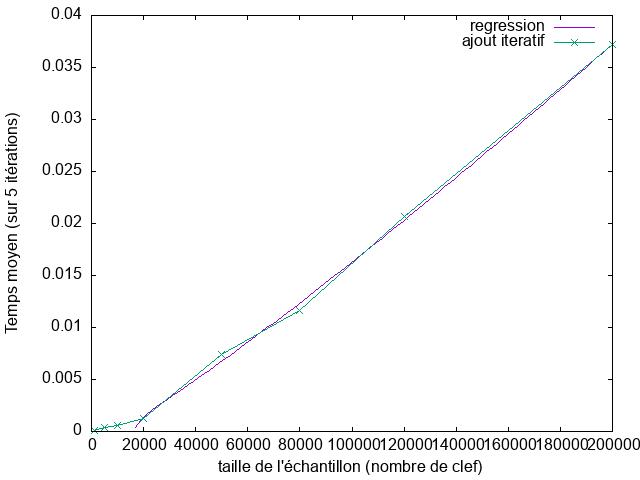
\includegraphics[scale=0.4]{../Images/Courbes utilisées pour le rapport/regression_ajout_iteratif_tab.png}
\caption{Mesure du temps pris par l'ajout itératif, tas sous forme de tableau}
\label{fig1}
\end{figure}

En observant la correspondance(\ref{fig1}), il apparaît que l'ajout itératif sur le tableau semble être en $O(n log n)$.


\subparagraph{Tas implémenté avec une arborescence}

Nous obtenons la courbe et les paramètres pour la régression suivants : 


\begin{center}
\begin{tabular}{|c|c|c|c|c|}
\hline
 & a & b & c & m\\
\hline
coefficient & 1.37702e-08 & 
9.99416e-05 & 
-3862.02 & 
1.13792e+06 \\
Erreur asymptotique & +/- 5.828e-08 & +/- 0.0006326 & +/- 4.284e+10   & +/- 1.275e+08\\
\hline
\end{tabular}
\end{center}


\begin{figure}[hbtp]
\centering
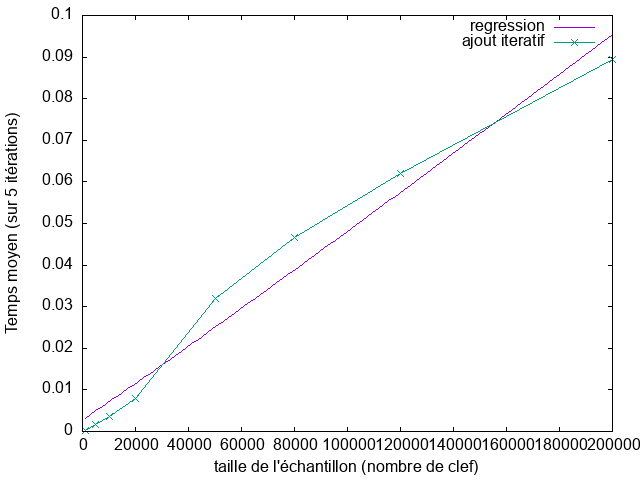
\includegraphics[scale=0.4]{../Images/Courbes utilisées pour le rapport/regression_ajout_iteratif_arbre.png}
\caption{Mesure du temps pris par l'ajout itératif, tas sous forme d'arbre}
\label{fig2}
\end{figure}

Notons ici (\ref{fig2}) que la régression linéaire est moins alignée avec nos différents points, mais la correspondance peut néanmoins nous faire considérer que l'ajout itératif implémenté par arborescence semble être en $O(n log n)$.




\subsubsection{Construction}

La complexité théorique de la fonction de construction, comme montré précédemment, est en $O(n)$, nous avons donc utilisé la fonction suivante pour l'ajuster à nos courbes avec les paramètres m et b : 

$$
f(x) = mx +b
$$

\subparagraph{Tas implémenté avec un tableau}

Nous obtenons la courbe et les paramètres pour la régression suivants : 

\begin{center}
\begin{tabular}{|c|c|c|}
\hline
 & m & b \\
\hline
coefficient & 3.38282e-07 & -0.00194051 \\
Erreur asymptotique & +/- 1.284e-08 & +/- 0.001147  \\
\hline
\end{tabular}
\end{center}


\begin{figure}[hbtp]
\centering
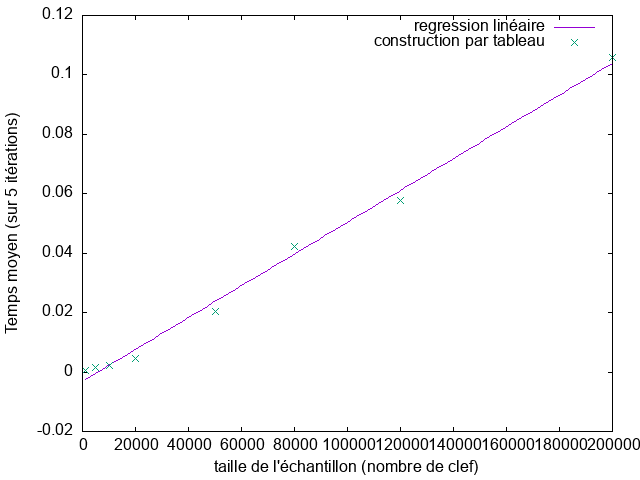
\includegraphics[scale=0.4]{../Images/Courbes utilisées pour le rapport/cplxt_cons_tab_regression.png}
\caption{Mesure du temps pris par la construction, tas sous forme de tableau}
\label{fig3}
\end{figure}

En observant la correspondance (\ref{fig3}), il apparaît que la construction avec des tas implémentés par un tableau semble être en $O(n)$.


\subparagraph{Tas implémenté avec une arborescence}

Nous obtenons la courbe et les paramètres pour la régression suivants : 


\begin{center}
\begin{tabular}{|c|c|c|}
\hline
 & m & b \\
\hline
coefficient & 1.16615e-07 & 0.000263775 \\
Erreur asymptotique & +/- 3.17e-09 & +/- 0.0002832  \\
\hline
\end{tabular}
\end{center}


\begin{figure}[hbtp]
\centering
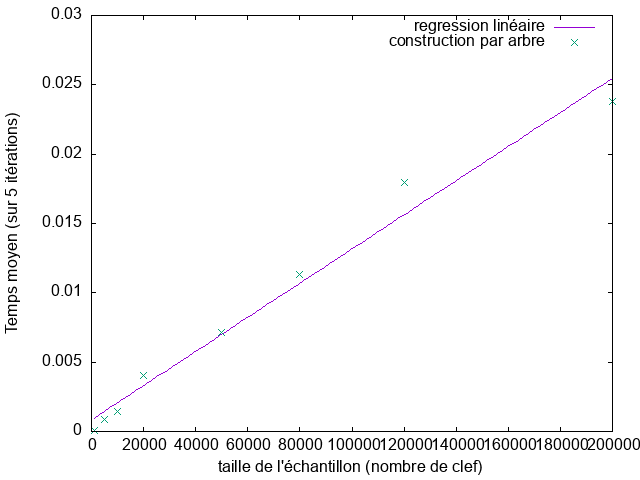
\includegraphics[scale=0.4]{../Images/Courbes utilisées pour le rapport/cplxt_cons_arbre_regression.png}
\caption{Mesure du temps pris par la construction, tas sous forme d'arbre}
\label{fig4}
\end{figure}

En observant la correspondance (\ref{fig4}), il apparaît que la construction avec des tas implémentés par une arborescence semble être en $O(n)$.




\subsubsection{Vérification graphique pour l'union}

La complexité théorique de la fonction de l'union, comme montré précédemment, est en $O(n + m )$, nous avons donc utilisé la fonction suivante pour l'ajuster à nos courbes avec les paramètres m et b ( $x = n+m $): 

$$
f(x) = mx +b
$$

Pour nos jeux de tests, nous avons décidé de faire fixer à chaque fois l'union entre deux tas de même taille. Nous courbes représentent donc l'évolution du temps par l'algorithme pour fusionner deux tas de taille n, variant de 1000 à 2000000,  20 itérations servent à faire la moyenne (pour nos 5 jeux de données d'une taille précise, on fait la fusion avec les autres jeux de données uns par uns). Ce choix est dû au fait que pour estimer la complexité au pire cas de l'union, la seule donnée intéressante à faire varier est $n+m$, avec n la taille du premier tas et m celle du second, et pas la taille des deux tas prise individuellement\footnote{De premiers essais en fixant $n$ à 1000 nous ont montré une complexité similaire, il ne nous a pas semblé utile d'aller plus loin dans les expérimentations sur ce sujet}.

Notons également d'une rapide vérification avec la commande unix diff nous a permis de nous assurer que dans nos jeux de clés de même taille, il n'y avait aucune répétitions.


\subparagraph{Tas implémenté avec un tableau}

Nous obtenons la courbe et les paramètres pour la régression suivants : 


\begin{center}
\begin{tabular}{|c|c|c|}
\hline
 & m & b \\
\hline
coefficient & 3.86017e-07 & -0.00183903 \\
Erreur asymptotique & +/- 7.759e-09 & +/- 0.000693  \\
\hline
\end{tabular}
\end{center}


\begin{figure}[hbtp]
\centering
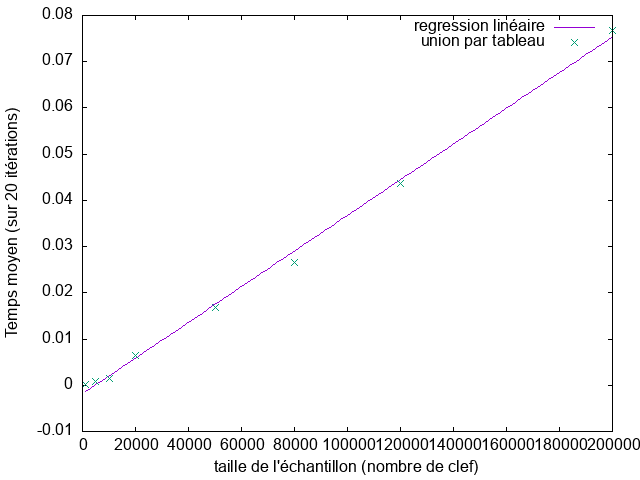
\includegraphics[scale=0.4]{../Images/Courbes utilisées pour le rapport/cplxt_union_tab_regression.png}
\caption{Mesure du temps pris par l'union, tas sous forme de tableau}
\label{fig5}
\end{figure}

En observant la correspondance (\ref{fig5}), il apparaît que l'union avec des tas implémentés par un tableau semble être en $O(n)$.


\subparagraph{Tas implémenté avec une arborescence}

Nous obtenons la courbe et les paramètres pour la régression suivants : 


\begin{center}
\begin{tabular}{|c|c|c|}
\hline
 & m & b \\
\hline
coefficient & 3.97294e-07 &-0.00070037 \\
Erreur asymptotique & +/- 6.106e-09 & +/- 0.0005454  \\
\hline
\end{tabular}
\end{center}


\begin{figure}[hbtp]
\centering
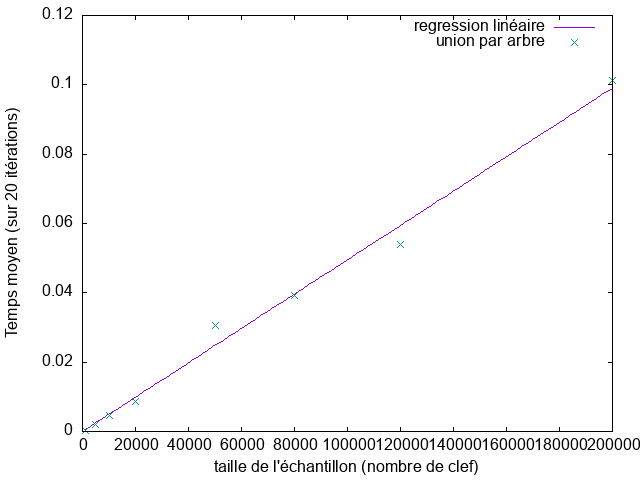
\includegraphics[scale=0.4]{../Images/Courbes utilisées pour le rapport/cplxt_union_arbre_regression.png}
\caption{Mesure du temps pris par l'union, tas sous forme d'arbre}
\label{fig6}
\end{figure}

En observant la correspondance (\ref{fig6}), il apparaît que l'union avec des tas implémentés par une arborescence semble être en $O(n)$.


\subsection{Conclusion sur cette partie}

Ainsi, dans cette section, nous avons étudié deux manières d'implémenter un tas minimal : la manière usuelle et impérative, et une manière davantage compatible avec le style fonctionnel d'OCaml.

Il est alors intéressant de noter que le choix du langage a probablement pu influencer nos expérimentations, notamment sur les vitesses des opérations dans nos deux structures : le tas minimal sous forme d'arbre semble être plus rapide, en OCaml, du fait que le langage s'adapte très bien au style fonctionnel\footnote{notre hypothèse concernant cette notable différence est que le compilateur optimise plus facilement cette manière de faire que des parcours de tableau}.

Grâce à l'implémentation purement fonctionnelle sous forme d'arbre, nous avons pu nous confronter aux difficultés qu'il peut y avoir à manipuler ce type de structures dans ce paradigme de programmation, ce qui nous a fait essayer de comprendre plus en détail le fonctionnement d'un tas, et de chercher des propriétés dessus qui pourraient nous être utiles pour parcourir nos arbres de haut en bas par un chemin en $O(log n)$.

Nous avons également pu étudier une manière moins naïve de construire un tas minimal grâce à l'algorithme de Robert Floyd\cite{ACM}, ainsi qu'une approche plus poussée de la complexité au pire cas sur des tas minimum.

\newpage
 \section{File binomiale}

Dans cette section, nous allons étudier l'implémentation en OCaml d'une file binomiale\cite{TasBinom}, et ce dans un style purement fonctionnel, ce qui s'accorde assez bien avec la structure.
Le code se trouve dans le fichier \textit{src/file\_binomiale}. Nous avons également ajouté une fonction \textit{to\_dot} permettant d'obtenir une représentation graphique de nos files binomiales, des exemples se trouvent dans \textit{Images/graphes}.

\subsection{Primitives et structure}

Nous définissions sa structure, en OCaml, à l'aide de deux types récursifs : 

\bigskip \begin{lstlisting}
(*Racine(degre,cle,fils)*)
type tournois_b = Racine of int * Int128.t * (tournois_b list)  | Empty 
(*File(indice,tournois) tournois le plus petit a gauche de la liste *) 
type file_b = File of int * (tournois_b list) | Empty 
\end{lstlisting} \bigskip

Nous définissons également les primitives suivante (leur code se trouve dans le fichier \textit{src/file\_binomiale.ml} :

\bigskip \begin{lstlisting}
let est_vide_t (t : tournois_b) : bool = (O(1))
let degree (t:tournois_b) : int = (O(1))
let union2Tid (t1:tournois_b) (t2:tournois_b) : tournois_b = (O(1))
let rec  pow_2 (n:int) : int = (O(1))
let decapiter (t: tournois_b) : file_b = (O(log n))
let file(t:tournois_b) : file_b = (O(1))
let est_vide_f (f: file_b ) : bool = (O(1))
let mindeg (f:file_b) : tournois_b = (O(1))
let reste (f:file_b) : file_b = (O(1))
let ajout_min (t:tournois_b) (f:file_b) : file_b = (O(log n))
\end{lstlisting} \bigskip

\subsection{Fonctions fondamentales}
Nous avons implémenté les fonctions fondamentales de manipulation d'une file binomiale conformément à leur définition dans le cours. L'implémentation étant assez transparente vis à vis du style fonctionnel utilisé en OCaml, nos fonctions sont assez transparentes avec les algorithmes sous-jacents.

Notons tout de même que la manière d'implémenter les files binomiales nous amène à avoir des tournois sous forme \texttt{[Empty]}, il a donc fallu traiter ce cas dans nos pattern matchings.

\subsubsection{Union}

La fonction Union est à réaliser en premier car elle est utilisée par toutes nos autres fonctions fondamentales : elle fonctionne de manière analogue à une addition bit à bit : on fusionne à chaque fois les tournois de degré identique pour former un tournoi du degré successeur, qui sera pris en compte comme une retenue pour la fusion suivante. Fusionner deux tas binomiaux de même taille consiste à faire d'un des deux tas le fils de la racine de l'autre (en gardant le minimum à la racine).

\bigskip \begin{lstlisting}

let rec unionFile (f1:file_b) (f2:file_b) : file_b =

  let rec uFret (f1 : file_b) (f2:file_b) (t:tournois_b) :file_b = 
    if est_vide_t t then  (* pas de tournois en retenu*)
      (*On fait la fusion des deux tas de meme degre en prenant la racine minimale comme parent de l'autre tas*)
      if est_vide_f f1 then f2
      else if est_vide_f f2 then f1 
      else
        let t1 = mindeg f1 in 
        let t2 = mindeg f2 in

        if (degree t1) < (degree t2) then ajout_min t1 (unionFile (reste f1) f2)
        else if (degree t2) < (degree t1) then ajout_min t2 (unionFile (reste f2)f1)
        else uFret (reste f1) (reste f2) (union2Tid t1 t2)


    else (*  t tournois en retenue *)
    	(*Meme principe, mais en prenant la retenue en compte*)
  in
  uFret f1 f2 Empty
\end{lstlisting} \bigskip


\subsubsection{Suppr\_min}

Pour supprimer le minimum, dans le cas où la file binomiale n'est pas vide, on utilise la fonction auxiliaire \textit{get\_min} qui nous permet d'obtenir une liste de tournois sans le minimum, ainsi que le tournois contenant le minimum. Il suffit alors de faire une union de la file binomiale sans le tournoi minimum, et le tournoi minimum privé de son élément minimal (qui est à sa tête).

\bigskip \begin{lstlisting}
let suppr_min (f:file_b) : file_b =
  match f with
  |Empty -> Empty
  |File(indice,tournois) ->   (*si la file est normal*)
    match tournois with
    |[]->Empty
    |Empty::tl -> Empty 
    |Racine(deg,cle,fils)::tl-> 
      let list_sans_min,tournois_min = get_min tournois cle in 
      (unionFile (File((indice - (pow_2  (degree tournois_min) )),list_sans_min)) (decapiter tournois_min))
      (* union entre la file privee de son tournoi min et de la file produite par le tournois min decapite*)
\end{lstlisting} \bigskip
\subsubsection{Ajout}

Pour réaliser l'ajout, il suffit de créer un tournoi contenant un tas binomial de degré 0 contenant l'élément à ajouter et de faire l'union avec la file binomiale passée en argument 

\bigskip \begin{lstlisting}
let ajout (x:Int128.t) (f:file_b) : file_b =
  let tx : tournois_b = Racine(0,x,Empty::[]) in
  let fx : file_b = file tx in
  unionFile f fx 
\end{lstlisting} \bigskip

\subsubsection{Construction}
On fait simplement des ajouts sucessifs dans la file qu'on créé :
\bigskip \begin{lstlisting}
let rec construction (liste_cles : Int128.t list): file_b =
  let rec loop (liste_cles : Int128.t list)  (file_bino : file_b) : file_b = 
    match liste_cles with 
    | [] -> file_bino
    | hd::tl -> (loop tl (ajout hd file_bino))
  in
  loop liste_cles Empty
\end{lstlisting} \bigskip


\subsection{Vérification graphique de la complexité de construction}
Ces expérimentations; et celles de la section suivante ont été faites selon le même protocole que pour le tas minimum. 

\begin{figure}[hbtp]
\centering
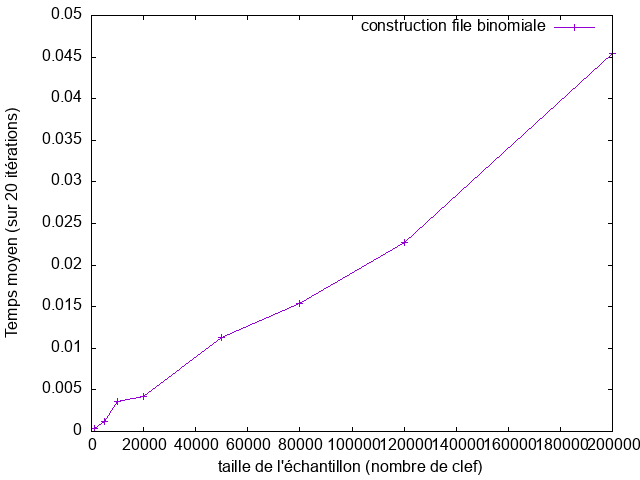
\includegraphics[scale=0.4]{../Images/Courbes utilisées pour le rapport/cplxt_binomiale.png}
\caption{Mesure du temps pris par la construction, file binomiale}
\label{fig7}
\end{figure}


La courbe (\ref{fig7}) obtenue expérimentalement semble confirmer notre complexité linéaire théorique.

\subsection{Vérification graphique de la complexité de union}

La complexité théorique de l'union de deux files binomiales est $O(log (n))$. Pour le vérifier, nous avons mesuré le temps que prenait l'union de deux files binomiales de taille égale, ce qui est un pire cas dans la mesure où il y a un nombre maximal de retenues à propager, ce qui prend le plus de temps dans notre algorithme.

\begin{figure}[hbtp]
\centering
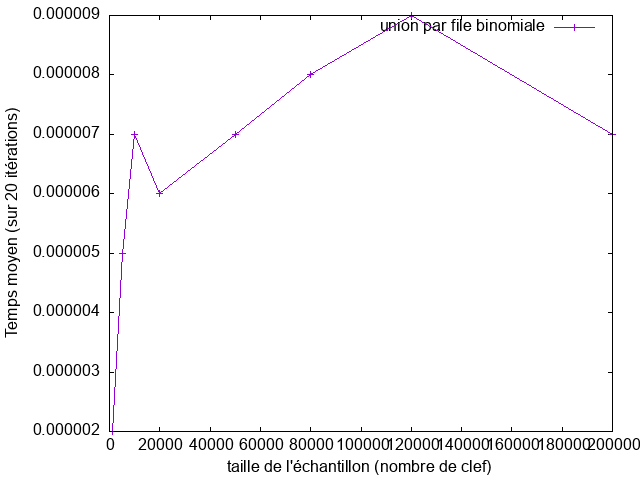
\includegraphics[scale=0.4]{../Images/Courbes utilisées pour le rapport/cplxt_union_file.png}
\caption{Mesure du temps pris par l'union de deux files binomiales de taille égale (en abscisse)}
\label{fig8}
\end{figure}


L'allure de la courbe (\ref{fig8}) semble bien nous indiquer une complexité en $O(log (n))$.


\subsection{Conclusion sur cette partie}

L'implémentation d'une structure de file binomiale se fait assez aisément en OCaml du fait de sa forme arborescente, nous avons pu ainsi implémenter cette structure et vérifier expérimentalement que nos fonctions s'approchaient des complexités théoriques souhaitées.

 \section{Hachage}

    Nous avons également choisi d'implémenter le hachage MD5\cite{md5} en OCaml. Nous aurions également pu utiliser un langage de plus bas niveau tel que le C permettant de manipuler simplement nos valeurs, mais nous avons préféré garder la cohérence du langage utilisé dans le projet plutôt que de faire de l'intégration\footnote{Notons que c'est cet autre choix qui a été fait dans la libraire standard de OCaml pour implémenter ces fonctions...} 

    \subsection{Représentation des valeurs}

    Nous avons choisit d'avoir comme entrée un argument de type string qu'on convertit ensuite en une liste de tableau de 16 entiers 32 bits. 
    Nous faisons ce choix car le MD5 travaille sur des blocs de 512 bits soit 16 entier 32 bits. A chaque tour de l'algorithme Nous travaillons donc sur un seul élément de cette liste de tableaux.

    \subsection{Traitement du messages} 
    \subsubsection{Transformation de la chaîne }
    
    Pour transformer notre string en int32 nous utilisons une fonction du module String qui permet de décoder bit a bit des int32 depuis des string :
    
\bigskip 
\begin{lstlisting}
    val get_int32_le : string -> int -> int32
\end{lstlisting} \bigskip  

    Cette fonction prend la chaîne et l'indice de début de l'entier a décoder en argument et renvoie une erreur si il reste moins de 32 bit a décoder (moins de 4 caractères).

    De plus la chaîne doit être paddée pour être divisible en bloque de 64 octets. 
    on doit ajouter un bit a 1 pour marqué la fin de la chaîne puis paddée avec des 0 jusqu'à ce qu'il reste 2 octets dans lesquels on stock la taille de la chaîne en bit sut 64 bits. 

    
    on ne va pas detailler cette transformation trivial a partir du moment ou on peu de transformer notre chaîne en entier.


    \subsubsection{implémentation du md5}
    
    Nous implémentons la fonction de hachage md5 en suivant l'algorithme classique. Nous avons également ajouté une fonction finish. Nous exécutons cette fonction sur les 4 int32 qui compose le int128 renvoyé par la boucle du md5 elle permet d'inverser les octets de l'entier, ici pour le ramener en little endian.
    
\bigskip \begin{lstlisting}
let finish (entre : int32) : int32 =
  let res = 0l in
  let res = Int32.logor res (Int32.shift_left (Int32.logand entre 0x000000FFl) 24) in 
  let res = Int32.logor res (Int32.shift_left (Int32.logand entre 0x0000FF00l) 8) in 
  let res = Int32.logor res (Int32.shift_right_logical (Int32.logand entre 0x00FF0000l) 8) in 
  let res = Int32.logor res (Int32.shift_right_logical (Int32.logand entre 0xFF000000l) 24) in 
  res
;;
\end{lstlisting} \bigskip 

    
\subsection{Conclusion sur cette partie}

Par cette manipulation fine des bits composant une chaîne de caractère, nous parvenons ainsi à hacher les chaînes passées en entrée pour obtenir des clés, ce qui nous permettra de transformer des textes pour en faire des listes de jeux de clé 128 bits, afin de tester les structures vues précédemment.

\newpage
 \section{Arborescence de Recherche}


Nous souhaitons dans cette partie implémenter une structure arborescente de recherche, avec la condition que la recherche dedans se fasse en un temps moyen de $log(n)$. Nous avons choisi comme structure répondant à cette condition un arbre 2-3-4\cite{234tree}, dans la mesure où la complexité des opérations d'ajout et de recherche sont en $O(log (n))$, et que son implémentation est plutôt facilitée dans le langage OCaml. 

Le code complet de cette section se trouve dans \textit{src/lib/arbre\_234.ml}. Nous avons également ajouté une fonction \textit{to\_dot} permettant d'obtenir une représentation graphique de nos files binomiales, des exemples se trouvent dans \textit{Images/graphes}.

\subsection{Définition de la structure}
Un arbre 2-3-4 est une structure arborescente de recherche définie comme suit :

\bigskip \begin{lstlisting}
type arbre234 = 
  | Empty
  | Feuille1 of Int128.t
  | Feuille2 of Int128.t * Int128.t
  | Noeud2 of Int128.t * arbre234 * arbre234 
  | Noeud3 of Int128.t * Int128.t * arbre234 * arbre234 * arbre234 
  | Noeud4 of Int128.t * Int128.t * Int128.t * arbre234 * arbre234 * arbre234 * arbre234 
\end{lstlisting} \bigskip 

Un $i-Noeud$ a $i$ fils et $i - 1$ clés, une $i-Feuille$ a $i$ clés. Notons qu'ici, les types sommes de OCaml nous permettent d'économiser l'espace, habituellement perdue en programmation en style impératif avec changement d'états, car nous ne stockons que le nombre de clés du i-Noeud dans chacun de nos constructeurs (et pas 3 en attendant de les remplir dans des structures mutables). 

Au sein de chaque $i-Noeud$, les $i-1$ clés nous permettent de nous aiguiller dans l'arborescence, l'ajout se fait toujours au niveau des feuilles.

Les arbres 2-3-4 ont la propriété d'avoir une hauteur en $O(log (n))$, ce qui nous assure les complexités souhaitées.


\subsection{Ajout dans la structure}
Afin d'ajouter des clés à notre structure, nous avons utilisé un mécanisme permis par OCaml, à savoir la levée d'exception pour remonter l'arbre des appels récursifs. On définit une exception \textit{Eclatement} qui permet de faire remonter une clé et deux sous-arbres :

\bigskip \begin{lstlisting}
exception Eclatement of (Int128.t * (arbre234) * (arbre234)) ;;
\end{lstlisting} \bigskip

Cette dernière est levée,  lorsqu'on cherche à ajouter une clé soit à une 2-Feuille, soit à un 4-Nœud. Dans ce cas là, on va faire remonter l'élément "central" dans nos 3 (resp. 4) clés selon l'ordre défini sur ces dernières avec pour fils deux sous-arbres correspondant à ce qu'il reste du nœud après éclatement.

À chaque appel récursif, on fait un motif \textit{try ... catch} permettant de rattraper le fait qu'un nœud ait été éclaté afin de reconstruire le nœud voulu (au besoin, on lève à nouveau une exception si on a de nouveau dû éclater un nœud).

\bigskip \begin{lstlisting}
(*On suppose que cle n'est pas dans t*)
let ajout (cle : Int128.t) (t : arbre234) : arbre234 = 
  let rec insertion234 (cle : Int128.t) (t : arbre234) : arbre234 = 
    if (est_dans_noeud cle t) then t 
    else
      match t with 
      | Empty -> Feuille1(cle)
      | Feuille1(elt) -> (* creation d'une Feuille2 contenant cle au bon endroit*)
      | Feuille2(elt1,elt2) -> 
        if (Int128.inf cle elt1) then 
          raise (Eclatement (elt1,Feuille1 (cle),Feuille1(elt2)))
        else if (Int128.inf cle elt2) then 
          raise (Eclatement (cle,Feuille1 (elt1),Feuille1(elt2))) 
        else 
          raise (Eclatement (elt2,Feuille1 (elt1),Feuille1(cle))) 
      | Noeud2 (elt, g,d) ->  
        if (Int128.inf cle elt) then 
          (try Noeud2 (elt,insertion234 cle g, d)
           with Eclatement (r,ng,nd) -> Noeud3(r,elt,ng, nd, d))
        else 
          (*resp. avec l'autre fils au centre *)
      | Noeud3 (elt1, elt2, g,m,d) -> (* idem 2Noeud mais avec une cle et un fils en plus*)

      | Noeud4 (elt1, elt2, elt3, g, m, n, d) ->
        if (Int128.inf cle elt1) then 
          (*Inserer a g et recuperer un possible eclatement*)
          ( try (Noeud4 (elt1, elt2, elt3, insertion234 cle g, m, n ,d))
            with Eclatement (r,ng, nd) -> 
              raise (Eclatement (elt2,Noeud3 (r, elt1,ng,nd,m), Noeud2 (elt3, n, d)))
          )
        else (*idem mais avec l'aiguillage approprie pour descendre vers les bonnes feuilles pour l'insertion*)
  in 
  match t with 
  (*Gestion des cas de base*)
\end{lstlisting} \bigskip

\subsection{Recherche dans l'arbre}
La recherche se fait alors en suivant à chaque nœud le chemin selon l'encadrement des clés du nœud, puisque la hauteur d'un arbre 234 est en $O(log(n))$, la recherche l'est aussi, puisqu'on ne parcourt qu'une branche ayant une longueur en $O(log (n))$.


\subsection{Conclusion sur cette partie}

Grâce à la structure des arbres 234, nous avons un moyen de stocker des clés, et de vérifier plutôt rapidement si elles y appartiennent, ce qui nous sera utile, combiné à notre fonction de hachage implémentée précédemment, afin d'établir une liste de clés unique pour un ensemble de textes données.

 \section{Étude expérimentale}

\subsection{Extraire la liste de mots}

Le code de cette sous section se trouve dans \textit{tests/liste\_mots.ml}. Une fonction sert à fabriquer 

Afin d'établir cette liste, nous utilisons la structure d'arbre définie dans la section précédente ainsi que la fonction de hachage de la section 4.

Une fonction auxiliaire nous permet d'ajouter à un accumulateur tous les mots d'un fichier à une liste en vérifiant qu'ils ne sont pris qu'une seule fois en les stockant au fur et à mesure dans un arbre de recherche. Nous avons également choisi de filtrer les mots apparaissant dans des didascalies ( '[' ou ']' apparaissant dans la ligne dans le fichier) afin de ne pas les compter deux fois.

Par un parcours de tous les fichiers du dossier grâce à la fonction \textit{readdir} du module \textit{Sys}, nous parvenons à ajouter à notre accumulateur tous les mots des différentes œuvres de façon unique. L'ajout se faisant en tête en OCaml, il nous suffit de renverser la liste à la fin afin d'avoir le premier mot en tête de liste et le bon ordre pour les autres.

La liste ainsi obtenue est composée de 22933 mots uniques\footnote{Nous avons fait le choix d'opter pour la cohérence vis à vis des données étudiées et de considérer que, par exemple, "[the" et "the" sont le même mot, en ne faisant pas ce filtrage, nous obtenons 23086 mots.} qui constitueront notre jeu de tests final pour nos structures. Afin de faciliter son utilisation, nous produisons directement une liste de clés de 128 bits obtenues grâce au hachage des mots. 

\subsection{Collisions par notre fonction de hachage sur l'échantillon}


Nous faisons la supposition que la fonction de hachage md5 est uniforme, en appliquant la formule du paradoxe des anniversaires, nous pouvons calculer la probabilité qu'il y ait des collisions pour les mots de notre texte :

\begin{align}
\mathbb{P} &= 1 - \prod_{i = 0}^{n -1} ( 1 - \frac{i}{m})\\
&= 1 - exp \prod_{i = 0}^{n -1} ln( 1 - \frac{i}{m})\\
&\approx 1 - e^{-\frac{n^2}{2m}}
\end{align}

En considérant m le nombre de valeurs possibles et n le nombre de valeurs à hacher, appliqués à notre cas, à savoir, dans le cas le plus extrême, les mots de la langue anglaise, on a :

\begin{itemize}
\item $m = 2^{128}$ (nombre de clés possibles codées sur 128 bits)
\item $n \approx 271000$ (nombre de mots de la langue anglaise)
\end{itemize}

On a alors 
$$\mathbb{P}\approx 1 - e^{-\frac{7,3441\times10^{10}}{2^{129}}} \approx 1,0791\times10^{-28}$$,

Cette probabilité étant très faible, alors que la supposition que Shakespeare a utilisé tous les mots de la langue anglaise est assez large, nous considérons qu'il n'y a pas de collisions.

\subsection{Comparaison de nos structures sur le jeu de données obtenu}

Le code de cette sous section se trouve dans \textit{tests/experimentation\_Shakespeare.ml}. Nous utilisons les fonctions du module \textit{Liste\_mots} afin d'obtenir la liste servant aux jeux de tests. Une fonction de formatage pour nos complexités a été ajoutée à \textit{manipulation\_fichiers.ml} pour faciliter l'écriture de nos mesures dans un fichier .txt pour utiliser gnuplot dessus.

\subsubsection{Construction}

Pour mesurer le temps pris pour chaque structure par la construction, nous utilisons la liste complète.

Nous obtenons les temps suivants :


\begin{figure}[hbtp]
\centering
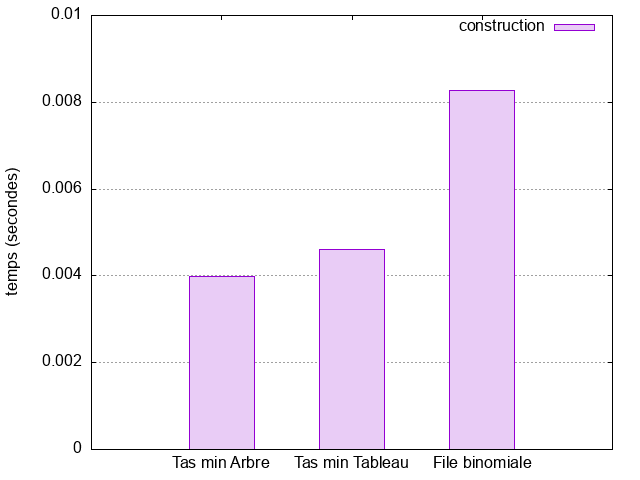
\includegraphics[scale=0.5]{../Images/Courbes utilisées pour le rapport/temps_construction_shakespeare.png}
\caption{Temps pris par la construction du jeu de données pour nos différentes structures}
\label{fig9}
\end{figure}

On remarque (\ref{fig9}) alors que le tas par arbre est légèrement plus efficace que par tableau, la file binomiale est significativement plus lente. Le léger avantage de l'arbre pourrait s'expliquer par le fait que manipuler un tableau de si grande taille n'est pas le plus optimal avec OCaml, vis à vis d'une structure purement fonctionnelle.


\subsubsection{Union}

Pour l'union, nous avons choisi de séparer notre liste en deux de manière aléatoire (une chance sur deux d'aller à gauche ou à droite avec \textit{Random.bool()} grâce à la fonction \textit{partition} du module \textit{List}. On souhaite ainsi obtenir deux structures où la répartition se rapprocherait du cas où on voudrait simplement fusionner deux tas sans avoir aucune propriété définie sur leur taille ou leur contenu (ordre des clés, taille, etc).


\begin{figure}[hbtp]
\centering
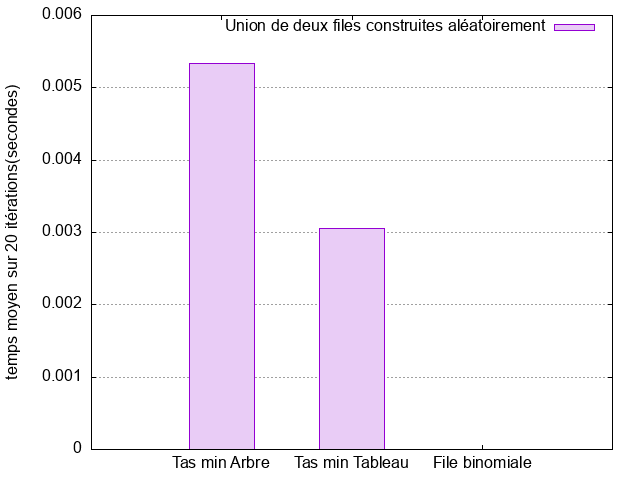
\includegraphics[scale=0.5]{../Images/Courbes utilisées pour le rapport/temps_union_shakespeare.png}
\caption{Temps pris par l'union pour nos différentes structures}
\label{fig10}
\end{figure}

On remarque alors deux choses (\ref{fig10}): 

\subparagraph{Le tas par arbre est plus lent que par tableau}, ce qui peut s'expliquer par le fait qu'on re-créé deux listes à partir de nos deux tableaux en $n+m$ opérations avant d'appliquer construction (en $O(n+m)$), là où pour le tableau, on utilise la fonction append qui nous permet directement d'avoir une forme d'arbre parfait tassé à gauche où utiliser l'algorithme de construction présenté en section 2.2.

\subparagraph{L'union par file "n'apparaît pas" dans notre histogramme} : en effet, le temps pris par l'union sur une file binomiale est beaucoup plus rapide que sur un tas ($O(log n)$), le temps mesuré est alors négligeable vis à vis des deux autres.

\subsubsection{Suppression du minimum}
Pour la suppression du minimum, nous le faisons sur les structures construites avec la fonction \textit{construction}.

\begin{figure}[hbtp]
\centering
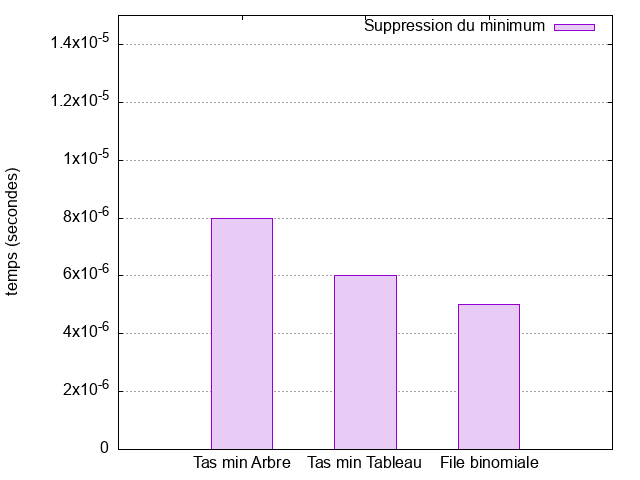
\includegraphics[scale=0.5]{../Images/Courbes utilisées pour le rapport/temps_suppr_shakespeare.png}
\caption{Temps pris par la fonction \textit{supprMin} sur nos différentes structures}
\label{fig11}
\end{figure}


Le temps pris par le tas sous forme de tableau ou sous forme d'arbre est équivalent, mais la suppression est plus rapide avec une file binomiale (\ref{fig11}).

\subsubsection{Ajout}

Pour mesurer le temps pris par l'ajout, nous avons choisi de construire nos structures avec le jeu de clés, en retirer le minimum, puis l'ajouter à nouveau : cela nous permet de mesurer un pire cas pour nos tas puisqu'ajouter l'élément minimum nous garantit de faire le plus d'échanges possibles étant donné que nous l'ajoutons aux feuilles du tas, et que pour respecter sa propriété minimum, l'algorithme va le remonter jusqu'à la racine.

\begin{figure}[hbtp]
\centering
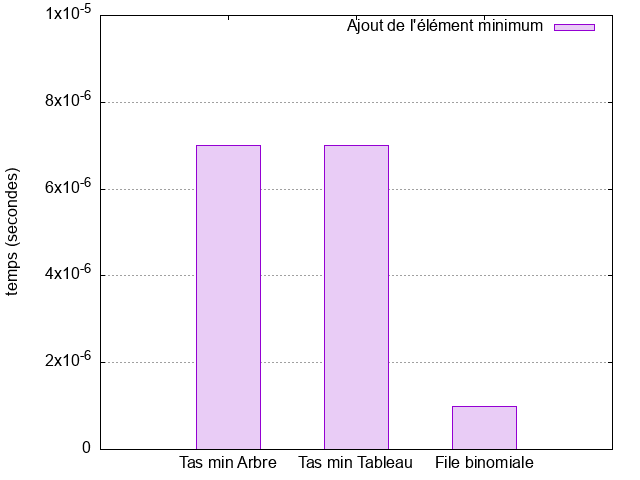
\includegraphics[scale=0.5]{../Images/Courbes utilisées pour le rapport/temps_ajout_shakespeare.png}
\caption{Temps pris par la fonction \textit{ajout} sur nos différentes structures}
\label{fig12}
\end{figure}

On remarque que le tas par arbre est légèrement plus rapide que le tas par tableau (\ref{fig12}). Cependant, la file binomiale reste plus rapide.


\subsection{Conclusion sur cette partie}

Ainsi, grâce aux jeux de données établi depuis des données réelles (les œuvres de Shakespeare), nous avons pu confronter nos différentes structures sur leurs fonctions de manipulation usuelles (construction, union, suppression du minimum et ajout). Il en ressort qu'aucune n'est meilleure que les autres sur toutes ces opérations, en revanche, hormis la construction, la file binomiale semble plus efficace en terme de temps.

\newpage

 \section{Conclusion sur le devoir de programmation}
 

\subsection{Comment exécuter le code}

Pour effectuer les tests, il suffit d'ouvrir un terminal dans le répertoire \textit{test/}.

\subparagraph{Obtenir des représentations graphiques de nos structures} : la commande \textit{make test\_graphique} permet la création des images grâce au langage dot (dans \textit{Images/graphes}. La variable {\scriptsize\textit{VAL\_TEST\_GRAPHIQUE}} de la commande make permet de changer de jeu de données pour faire les graphes, et le nombre de nœuds souhaités.

\subparagraph{Mesurer le temps pris par nos fonctions} : la commande \textit{make test\_temps} permet de réaliser nos tests de complexités et d'obtenir nos courbes dans \textit{Images/courbes} avec un script gnuplot.

\subparagraph{Expérimentation sur l'œuvre de Shakespeare} : la commande \textit{make exeprimentation\_shakespeare} permet de réaliser nos mesures sur le jeu de données obtenus dans la section 6 dans \textit{Images/courbes\_shakespeare} avec un script gnuplot.


\subsection{Bilan}

Ce devoir nous auras ainsi permis d'une part d'étudier la manière dont on peut implémenter des algorithmes étudiés en cours sous forme de pseudo code, et donc de voir quelles adaptations sont parfois nécessaires pour une mise en œuvre effective sur machine.

L'utilisation du langage OCaml nous a également permis de réfléchir à la manière dont le paradigme de programmation utilisé influence la manière dont une structure et un algorithme seront implémentés.  Plus précisément, étudier une représentation, non usuelle, des tas sous forme arborescente nous a permis d'étudier comment adapter de manière purement fonctionnelle une structure de données dont le principe d'implémentation classique est très impératif.

Les études expérimentales nous ont permis d'étudier le temps réel pris par nos algorithmes et de voir que ce dernier s'approchait des complexités théoriques calculées.

Les trois dernières parties nous ont permis d'étudier comment mettre en place un jeu de données tiré d'exemples réels afin de comparer l'efficacité de nos différentes structures sur des manipulations usuelles. La réalisation de ces expériences nous a alors montré qu'il n'y a pas de structures parfaites étant meilleure sur toutes les opérations : le choix d'une structure plutôt qu'une autre pour répondre à un problème doit avant tout être fait en fonction de quelle opération sera le plus souvent effectuée. 


\cleardoublepage

\addcontentsline{toc}{section}{Bibliographie}
\bibliography{biblio.bib}
\bibliographystyle{plain}


\end{document}
